% !TEX program = pdflatex
\documentclass[3p,11pt]{elsarticle}
\usepackage{amsmath,amssymb}
\usepackage{array}
\usepackage{booktabs}
\usepackage[tableposition=top]{caption}
\usepackage{enumitem}
\usepackage{graphicx}
\usepackage{tikz}
\usepackage{pgfplots}
\usepgfplotslibrary{groupplots}
\pgfplotsset{compat=1.18}
\usepackage{url}
\urlstyle{same}
\usepackage[hidelinks]{hyperref}
\emergencystretch=3em
% first-page footer: the page number alone
\makeatletter
\def\ps@pprintTitle{\let\@oddhead\@empty\let\@evenhead\@empty
  \def\@oddfoot{\hfil\thepage\hfil}\let\@evenfoot\@oddfoot}
\makeatother
% a table body read from a file, expandable so that a rule may follow it
\makeatletter
\newcommand{\tabinput}[1]{\@@input #1 }
\makeatother

% ---- notation ---------------------------------------------------------------
\newcommand{\kms}{km\,s$^{-1}$}
\newcommand{\Msun}{M$_\odot$}
\newcommand{\Kone}{$K_1$}
\newcommand{\Ktwo}{$K_2$}
\newcommand{\dvsys}{$\Delta v_\mathrm{sys}$}

\begin{document}

\begin{frontmatter}

\title{Double-lined from the archive: independent dynamical masses of M dwarfs in eclipsing binaries from public HARPS and ESPRESSO spectra}

\author{Charles C. Norton}

\begin{abstract}
An eclipsing binary of a solar-type star and an M dwarf gives model-independent masses for both
stars once the M dwarf's own lines are measured, at optical flux ratios near $10^{-3}$. This paper
measures them from public ESO archive spectra with an analysis built independently of the published
ones. The spectra are placed in the primary's frame at their measured velocities and divided by
their series' median, cross-correlated with an empirical M1\,V spectrum, cleaned of the star's and
the sky's patterns and of five principal components, and summed along the companion's track over
its semi-amplitude \Ktwo\ and its systemic offset. Each summit is set against $10^4$ draws of two
nulls, the orbit's phase moved and whole nights shuffled, with a Gumbel law for the tail, and the
35 binaries of the survey are accounted for together. TOI-1338/BEBOP-1 (260 ESPRESSO spectra), EBLM
J0310$-$31 (114 HARPS spectra) and HD\,4875 (35 HARPS spectra) give false-alarm probabilities of
$10^{-11}$, $8\times10^{-12}$ and $1\times10^{-8}$ and \Ktwo\ $= 77.27 \pm 0.10 \pm 0.15$, $88.12
\pm 0.18 \pm 0.34$ and $75.29 \pm 0.30 \pm 0.87$\,\kms\ (statistical, then systematic from the
series' parts by date and its seasons), against published values of $77.16 \pm 0.48$, $88.27 \pm
0.46$ and $75.13 \pm 0.16$\,\kms; HD\,4875's companion had been measured only in the
near-infrared. The companion's lines sit $+1.05$ to $+1.25$\,\kms\ from the primary's systemic
velocity. Among the 35 southern EBLM binaries with archived HARPS series, one further companion
stands with a false-alarm probability of $1.5\times10^{-7}$ across the whole survey: EBLM
J2101$-$45, whose 75 spectra give \Ktwo\ $= 65.41 \pm 0.32 \pm 0.32$\,\kms\ and minimum masses of
$1.415$ and $0.552$\,\Msun, stable under changes of template, band and principal components and
recovered when a companion is injected into the same spectra. J0649$-$27, J0825$-$67 and J1141$-$37
reach 3.3 to $3.9\sigma$ alone but 2.1 to $3.0\sigma$ across the survey, and remain candidates.
Among 41 further EBLM binaries whose orbits are fitted to their own HARPS velocities, the
companions of J2122$-$32, J0425$-$46, J2054$-$32 and J0535$-$08 stand at 5.3 to $5.7\sigma$ across
the 41 and four more are candidates. NIRPS spectra recover J1540$-$09's published companion at
\Ktwo\ $= 59.98 \pm 0.50 \pm 0.78$\,\kms\ and give a candidate in J1613$-$76, whose HARPS series
shows none, and the TESS eclipses turn nine of these binaries' minimum masses into masses and
radii, J0535$-$08's $0.970 \pm 0.011$ and $0.521 \pm 0.003$\,\Msun.
\end{abstract}

\begin{keyword}
Binaries: eclipsing \sep Binaries: spectroscopic \sep Stars: low-mass \sep
Stars: fundamental parameters \sep Techniques: radial velocities
\end{keyword}

\end{frontmatter}

\section{Introduction}\label{sec:intro}

Masses and radii of M dwarfs set the properties inferred for the planets that orbit them, and
the empirical relations behind those inferences rest on stars whose masses are measured
without models. Detached double-lined eclipsing binaries provide such masses, but few are
known below the fully convective boundary near 0.35\,\Msun~\cite{Torres2010,Southworth2015},
since an M dwarf paired with a solar-type star contributes about a thousandth of the optical
light and its lines are lost in the primary's. The EBLM project has characterised hundreds of
these single-lined eclipsing binaries~\cite{Triaud2013,Triaud2017,Maxted2023}, measuring the
primary's spectroscopic orbit and the eclipses and taking the primary's mass or radius from
stellar models. The BEBOP survey for circumbinary planets has added years of precise velocities
of the same stars with HARPS and SOPHIE~\cite{Martin2019,Standing2022,Triaud2022}.

The secondary's lines can nonetheless be recovered. High-resolution cross-correlation, developed
to detect molecules in exoplanet atmospheres~\cite{Snellen2010,Brogi2012}, sums a weak spectrum
along a known orbit after the stationary spectrum has been removed. Sebastian et al.\ applied it
to the circumbinary planet host TOI-1338/BEBOP-1~\cite{Kostov2020,Standing2023} and detected its
M dwarf at $11\sigma$ in 103 ESPRESSO spectra, measuring \Ktwo\ $= 77.16 \pm 0.48$\,\kms\ and
masses of $1.098 \pm 0.017$ and $0.307 \pm 0.003$\,\Msun~\cite{Sebastian2024b}, with the
Saltire model of the cross-correlation map~\cite{Sebastian2024a}. The method has since been
applied to Kepler-16 with SOPHIE~\cite{Sebastian2025b}, to BEBOP-3~\cite{Baycroft2025} and to
five more EBLM binaries, among them EBLM J0310$-$31~\cite{Stevenson2026}. In the near-infrared,
where the M dwarf is relatively brighter, the secondary's semi-amplitude has been measured with
SPIRou~\cite{Maxted2022}, CRIRES+~\cite{Sebastian2025a} and NIRPS~\cite{Adshead2026,Hahlin2026}.

These measurements share a small number of analysis designs, and their accuracy has been tested
by splitting each dataset in time and by simulation~\cite{Sebastian2024b,Stevenson2026}. An
analysis built independently, with a different template, a different removal of the primary's
spectrum and a different measure of significance, tests that accuracy from outside. The public
archives also hold more spectra of these stars than the published analyses used: the ESO archive
holds 114 HARPS spectra of EBLM J0310$-$31 above a signal-to-noise ratio of 10, against the 71 of
ref.~\cite{Stevenson2026}, and 264 ESPRESSO spectra of TOI-1338, against 103.

This paper describes such an analysis, the binaries approach of the seti-tools package, which
shares its spectra machinery with the package's planet-frame and free-orbit companion searches and
their orbitlight release~\cite{orbitlight}, and applies it to public products of the ESO Science
Archive alone. Section~\ref{sec:data} selects the targets and spectra and
Section~\ref{sec:method} describes the method, its statistic and its calibration.
Section~\ref{sec:validation} compares its results for three systems with published dynamical
masses, which test its accuracy, its uncertainties and its false-alarm probabilities.
Section~\ref{sec:survey} applies it to the southern EBLM binaries with HARPS series and separates
the one new measurement from the candidates. Section~\ref{sec:wider} extends it to EBLM binaries
whose orbits come from their own spectra, to NIRPS spectra and to the TESS eclipses, and
Section~\ref{sec:discussion} discusses what the comparison shows.

\section{Targets and spectra}\label{sec:data}

The targets are the single-lined spectroscopic binaries with archived high-resolution spectra.
The Gaia DR3 non-single-star catalogue~\cite{GaiaNSS2023} gives 203\,121 single-lined orbits
(solution types SB1, SB1C and AstroSpectroSB1) for stars brighter than $G = 13$, and the SB9
catalogue~\cite{Pourbaix2004} 3\,426 single-lined orbits. Each was matched within
10\,arcsec to the ESO archive's series of 20 or more spectra of one target from HARPS, ESPRESSO,
NIRPS, UVES or FEROS, giving 140 series of 126 stars. A series is searched when its orbit has a
period below 100\,d covered three or more times, the series holds 30 or more spectra, and the
mass function allows a companion of 0.07\,\Msun\ or more around a primary of 1\,\Msun. That
leaves 68 series. Among them are the HARPS series of 37 EBLM binaries, named here by their EBLM
designations, which this paper searches, and TOI-1338's ESPRESSO series; the others belong to O and
B stars, interacting binaries with compact companions, and solar-type binaries observed mostly with
UVES or FEROS.

The spectra are the archive's Phase 3 one-dimensional products, with barycentric wavelengths and
the pipeline's flux and error. For each series, every product with a signal-to-noise ratio above
10 is taken, up to 300 spread evenly over the series' span.

\section{Method}\label{sec:method}

\subsection{The primary's velocities and orbit}

Each spectrum is placed on a grid uniform in velocity at 1\,\kms\ from 3800 to 7880\,\AA,
divided by its running median over 501 samples, with the telluric bands removed. Its velocity is
the peak of its cross-correlation over $\pm 200$\,\kms\ with the line depths of a G0\,V template,
one minus the median of EBLM J0310$-$31's 114 HARPS spectra placed at their velocities on its
Gaia orbit, refined by a parabola through the three highest samples. The primary's orbit is fitted
to these velocities in two steps. A grid over period (within 0.4 per cent of the catalogue's, in
steps that move the last epoch by a fiftieth of an orbit), phase (in hundredths), eccentricity (to
0.6) and argument of periastron (in $20^\circ$ steps) is searched with \Kone\ and the systemic
velocity $\gamma$ solved linearly at each point, and the best point starts a least-squares fit with
a soft loss in period, time of periastron, $\sqrt{e}\cos\omega$, $\sqrt{e}\sin\omega$, \Kone\ and
$\gamma$. The grid makes the fit independent of errors in the catalogue orbit, which for
TOI-1338 put the period 0.021\,d long and $\omega$ $58^\circ$ away.

\subsection{Residuals in the primary's frame}

Each spectrum is then moved into the primary's frame at its own measured velocity, placed on the
same grid, divided by its running median and by the series' median spectrum, and a cubic in
wavelength is removed. A residual shift of a spectrum against the median of 0.5\,\kms\ or more is
taken out before the division. The telluric bands and the sodium sky lines at their telescope
wavelengths are masked. Each wavelength's scatter across the series, floored at a tenth of its
median, weights the cross-correlation.

\subsection{Cross-correlation with an M-dwarf template}

The template is an empirical M1\,V spectrum: the line depths, one minus the median, of the archived
HARPS spectra of GJ\,367~\cite{Lam2021} in its own frame, negative values set to zero. Each
residual is cross-correlated with it by inverse variance over $\pm 300$\,\kms\ at 1\,\kms, the
result normalised so that a residual of unit noise gives unit scatter. Each cross-correlation row
then loses three patterns that are not the companion's: the star's own residual pattern, the
median row fitted to each row within 40\,\kms\ of the star and subtracted; the sky's pattern, the
rows' median in the telluric frame fitted back to each row; and five principal components of the
rows, which carry the shapes the star's pattern takes from night to night. Each row is weighted by
the inverse square of its robust scatter more than 50\,\kms\ from the star.

\subsection{The sum along the companion's track}

The companion's barycentric velocity at time $t$ is
\begin{equation}
v_2(t) = \gamma + \Delta v_\mathrm{sys} - K_2\left[\cos(\nu + \omega) + e\cos\omega\right],
\end{equation}
with $\nu$, $\omega$ and $e$ from the primary's fitted orbit and \dvsys\ the offset of the
companion's lines from the primary's systemic velocity. With $C_i(v)$ the cleaned
cross-correlation of spectrum $i$ at velocity $v$ in the frame in which it was placed,
$v_{\star,i}$ the velocity at which it was placed and $w_i$ its weight, the trail's value is
\begin{equation}
S(K_2, \Delta v_\mathrm{sys}) = \frac{\sum_i w_i\, m_i\, C_i\!\left(v_2(t_i) - v_{\star,i}\right)}{\sum_i w_i\, m_i},
\end{equation}
read by linear interpolation, where $m_i$ is one when the reading lies more than 30\,\kms\ from the
primary's lines and more than 10\,\kms\ from the row's telluric velocity and zero otherwise. $S$ is
defined where the readings number at least a fifth of the rows and at least ten. The map of $S$
over \Ktwo\ from \Kone\ to 160\,\kms\ and over \dvsys\ from $-30$ to $+30$\,\kms, both at
0.5\,\kms, gives the peak within 5\,\kms\ of zero offset, refined on grids of 0.1 and then
0.05\,\kms.

\subsection{The statistic and its false-alarm probability}\label{sec:stat}

The search statistic is the summit $\hat S = \max_{K_2} S$ over a grid from \Kone\ to 250\,\kms\
in steps of 0.25\,\kms, either at a fixed offset or, with the offset free, over the offsets within
5\,\kms\ of zero in steps of 0.5\,\kms\ as well. A null draw computes the same summit with the
companion's track replaced, by the orbit's phase moved by a uniform 0.1 to 0.9 of a period or by
whole nights moved to other nights' dates, each night keeping its spectra's offsets from its start,
so that what is tied to the orbital phase and what is tied to the hour or the night both stay in a
null. Each binary is set against $10^4$ draws of each null, $\hat S^{(j)}$, and three numbers
describe its summit. The first is its height in units of the nulls' scatter,
\begin{equation}
z = \frac{\hat S - \langle \hat S^{(j)} \rangle}{\mathrm{sd}(\hat S^{(j)})},
\end{equation}
a standardised statistic rather than a probability. The second is the empirical false-alarm
probability, $p_\mathrm{emp} = (1 + n_\ge)/(10^4 + 1)$, with $n_\ge$ the draws at or above $\hat
S$, which cannot fall below $10^{-4}$. The third extends the nulls with a tail model. Each null
summit is the largest of many correlated values of the trail, so the summits follow an
extreme-value law, and the Gumbel law~\cite{Gumbel1958} with the nulls' mean and scatter gives
\begin{equation}
p_\mathrm{G} = 1 - \exp\!\left\{-\exp\!\left[-\frac{\hat S - \mu}{\beta}\right]\right\},\qquad
\beta = \frac{\sqrt{6}}{\pi}\,\mathrm{sd}(\hat S^{(j)}),\quad \mu = \langle \hat S^{(j)} \rangle - 0.5772\,\beta .
\end{equation}
The null of the two with the larger $p_\mathrm{G}$ is adopted, and $p_\mathrm{G}$ is quoted with
the one-sided Gaussian significance of the same probability. A generalised extreme-value law fitted
to the same draws~\cite{Coles2001} measures the tail's shape $\xi$: zero for Gumbel's, negative for
a lighter tail, for which $p_\mathrm{G}$ overstates the probability, and positive for a heavier one.

The 35 searched binaries are accounted for together. In each draw of a null, the highest of the 35
binaries' summits, each in units of its own nulls' scatter, gives one draw of the survey's highest
null, and each binary's $z$ is set against these draws with a Gumbel law fitted in the same way.
Beside it, each binary's own $p_\mathrm{G}$ is compounded over the 35~\cite{Sidak1967},
$1 - (1 - p_\mathrm{G})^{35}$. The larger of the two, under the null that gives the larger, is the
false-alarm probability across the survey. A companion is taken as detected when its own
$p_\mathrm{G}$ reaches $5\sigma$ ($2.9\times10^{-7}$), and the probability across the survey is
quoted beside it.

\subsection{Uncertainty and masses}\label{sec:uncertainty}

The statistical uncertainty of \Ktwo\ is half the 16th to 84th percentile range of 300 draws of
whole nights with replacement, each cleaned again and its peak found on grids of 0.25 and then
0.05\,\kms. Noise that persists over a season is not in it. As in the published
analyses~\cite{Sebastian2024b,Stevenson2026}, each series is divided by date into four parts of
about equal numbers of spectra (two parts below 60 spectra), whole nights kept together, each part
cleaned and measured alone, and the parts' standard error with Bessel's correction is a systematic
uncertainty. The series is also resampled by observing season, runs of nights without a gap
longer than 90\,d, in 300 draws of whole seasons with replacement when it spans four seasons or
more. The larger of the two is the systematic uncertainty, added in quadrature to the statistical
one for the masses, which follow from
\begin{equation}
M_{1,2}\sin^3 i = 1.0361\times10^{-7}\,(1-e^2)^{3/2}\,(K_1+K_2)^2\,K_{2,1}\,P ,
\end{equation}
with the velocities in \kms, the period in days and the masses in \Msun, divided by $\sin^3 i$ at
the published inclination from the eclipses.

\subsection{Robustness tests}\label{sec:robust}

Each companion is measured again under five changes of the analysis: three and eight principal
components in place of five; the M-dwarf template kept only blueward or only redward of 5500\,\AA;
and the template made instead from the 110 archived HARPS spectra of L\,98-59, an M3 dwarf with
the same instrument~\cite{Cloutier2019}, in the same way as GJ\,367's. The band and template
changes rebuild the rows from the spectra. A synthetic companion is also laid into the actual
spectra before any processing: the template's lines at a V-band flux ratio of $10^{-3}$, and for
the four companions of Section~\ref{sec:survey} also $3\times10^{-4}$, scaled in wavelength as the
ratio of 3400 and 6000\,K black bodies, moving at the measured \Ktwo\ and an offset of $+1.0$\,\kms\
on the primary's orbit but a quarter of a period later than the real companion, so that the two
tracks cross only twice an orbit. The injected spectra go through the whole analysis and are read
along the moved track, the null with the phase moved kept a tenth of a period from the real
companion's track. The ratio of the real companion's peak to the injected one's at $10^{-3}$ gives
the flux ratio at which the real companion's lines match the template's.

\section{Three systems with published dynamical masses}\label{sec:validation}

Three of the binaries have published measurements of the secondary's semi-amplitude from other
data or other methods: TOI-1338 (EBLM J0608$-$59), measured from ESPRESSO spectra with
Saltire~\cite{Sebastian2024b}; EBLM J0310$-$31, measured from HARPS spectra with
Saltire~\cite{Stevenson2026}; and HD\,4875 (EBLM J0050$-$18), measured from NIRPS spectra by
cross-correlation with a synthetic M-dwarf spectrum~\cite{Hahlin2026}. The archive holds 264
ESPRESSO spectra of TOI-1338 above the signal-to-noise cut, of which 260 load, 114 HARPS spectra of
J0310$-$31 and 35 of HD\,4875. They test the method's accuracy, its uncertainties and the
calibration of its false-alarm probabilities on companions whose semi-amplitudes are known.

\subsection{Orbits}

The orbits fitted to the measured velocities (Table~\ref{tab:orbits}) leave a scatter of 14, 15
and 29\,m\,s$^{-1}$, which is the precision of a cross-correlation velocity against a template
built from one star's spectra, and they agree with the published orbits to within
$0.012$\,\kms\ in \Kone\ and $0.0003$ in eccentricity. The systemic velocities differ from the
published ones by 0.01 to 0.14\,\kms, the offset between the template's zero point and those of the
published analyses, which enters the companion's track only through \dvsys.

\begin{table}[t]
\centering
\caption{The primary's orbits fitted to the velocities measured here, against the published orbits.
$\omega$ is the primary's argument of periastron; rms is the scatter of the velocities about the
fit.}\label{tab:orbits}
\begin{tabular}{llrrrrr}
\toprule
System & Source & $P$ (d) & \Kone\ (\kms) & $e$ & $\omega$ ($^\circ$) & rms (m\,s$^{-1}$)\\
\midrule
TOI-1338  & this work & 14.608560 & 21.616 & 0.1556 & 117.86 & 14\\
          & ref.~\cite{Sebastian2024b} & 14.6085579 & 21.604 & 0.1555 & 117.77 & \\
J0310$-$31 & this work & 12.642791 & 27.868 & 0.3089 & 185.83 & 15\\
          & ref.~\cite{Stevenson2026} & 12.6427926 & 27.875 & 0.3087 & 185.85 & \\
HD\,4875  & this work & 13.635615 & 29.736 & 0.1814 & 251.71 & 29\\
          & ref.~\cite{Hahlin2026} & 13.6355611 & 29.739 & 0.1811 & 252.03 & \\
\bottomrule
\end{tabular}
\end{table}

\subsection{The companions}

The companion stands out in each system's map (Fig.~\ref{fig:maps}) at the published \Ktwo\ and
just redward of the primary's systemic velocity, and the trail over \Ktwo\ at that offset rises
alone above the nulls (Fig.~\ref{fig:curves}). Table~\ref{tab:k2} sets the results against the
published ones. The semi-amplitudes differ from the published values by $+0.11$, $-0.15$ and
$+0.16$\,\kms, which is 0.2, 0.3 and 0.2 times the two uncertainties combined, and at the published
inclinations the masses agree within 0.6 per cent. HD\,4875's published value comes from
near-infrared spectra alone.

The summits stand 19.3, 19.4 and 13.8 times the nulls' scatter above their mean, where the highest
of the adopted null's $10^4$ draws reaches 3.1, 5.2 and 3.0 times. No draw comes within reach of
the observed summits, so the empirical probabilities are at their floor of $10^{-4}$, and
the Gumbel law gives $10^{-11}$, $8\times10^{-12}$ and $1\times10^{-8}$, or 6.7, 6.7 and
$5.6\sigma$ (Table~\ref{tab:calib}). With the offset free within 5\,\kms\ of zero they are
$2\times10^{-12}$, $3\times10^{-10}$ and $2\times10^{-7}$. Across the survey's 35 binaries,
J0310$-$31 stays at $3\times10^{-10}$ ($6.2\sigma$) and HD\,4875 at $4\times10^{-7}$ ($4.9\sigma$).
The profile of the summed rows in the companion's frame (Fig.~\ref{fig:profiles}) is a single line
5 to 6\,\kms\ wide at half maximum, and nothing beyond 15\,\kms\ of it rises above three times the
profile's scatter.

\begin{table}[t]
\centering
\caption{The secondary's semi-amplitude, with its statistical and systematic uncertainties
(Section~\ref{sec:uncertainty}), the companion's systemic offset with the 16th to 84th percentiles
of 300 draws of whole nights, the summit at an offset of $+1.0$\,\kms\ in units of its nulls'
scatter with its false-alarm probability (Section~\ref{sec:stat}), and the masses at the published
inclinations, $89.639^\circ$, $86.531^\circ$~\cite{Stevenson2026} and
$89.057^\circ$~\cite{Hahlin2026}, against the published values.}\label{tab:k2}
\small\setlength{\tabcolsep}{4pt}
\begin{tabular}{lccc}
\toprule
 & TOI-1338 & J0310$-$31 & HD\,4875\\
\midrule
\tabinput{data/tab_k2.tex}
\bottomrule
\end{tabular}
\end{table}

\begin{figure}[t]
\centering
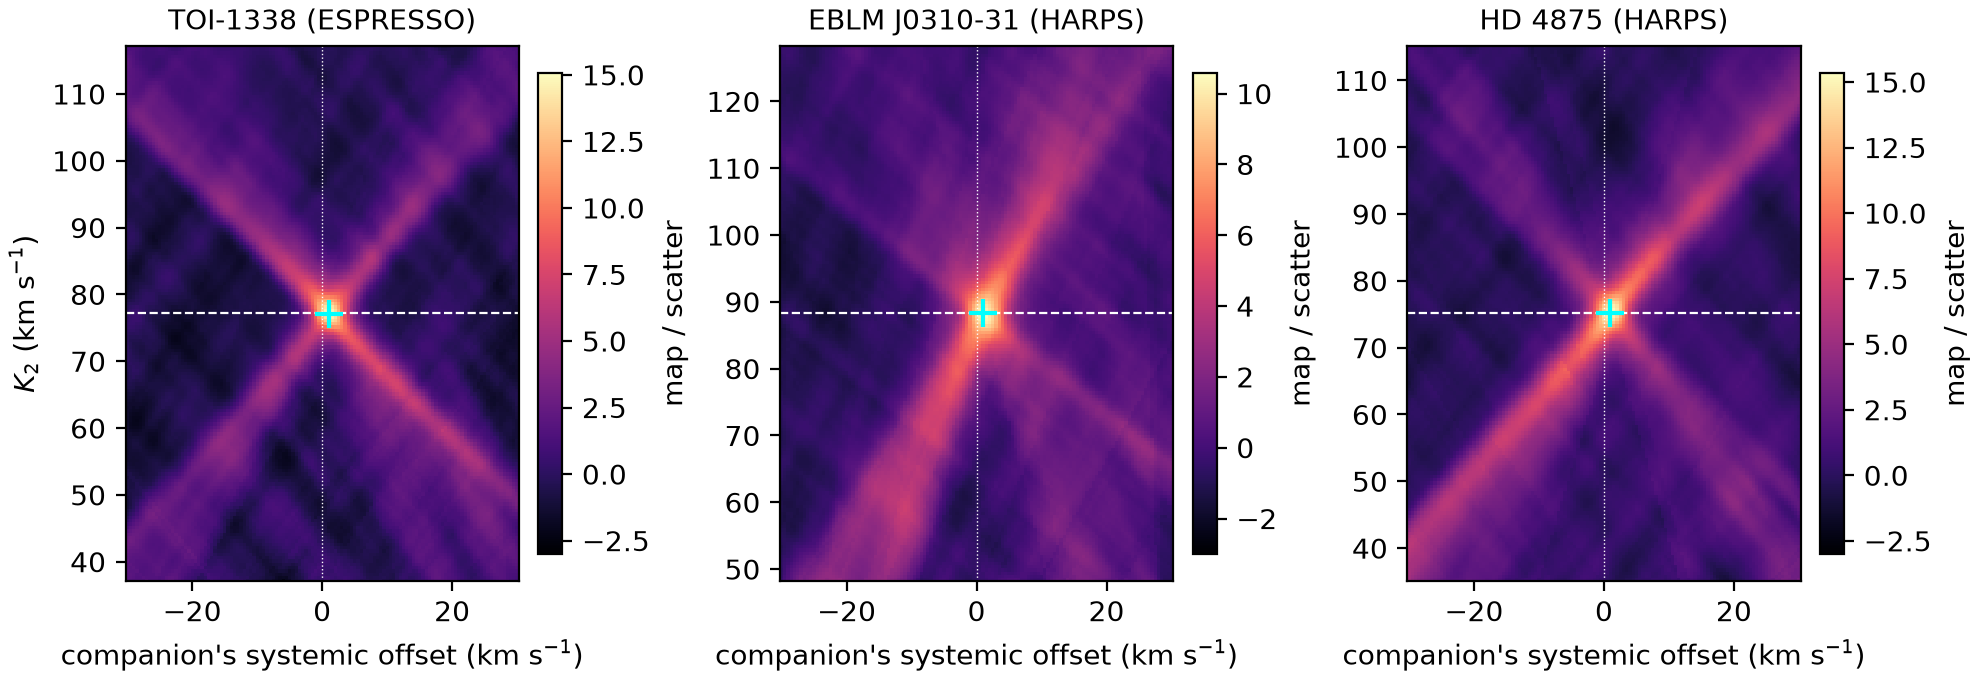
\includegraphics[width=\textwidth]{data/maps.png}
\caption{The mean of the cleaned rows along the companion's track over \Ktwo\ and the companion's
systemic offset from the primary's, in units of the map's scatter away from the peak. The dashed
line marks the published \Ktwo, the dotted line zero offset and the cross the peak.}\label{fig:maps}
\end{figure}

\begin{figure}[t]
\centering
\begin{tikzpicture}
\begin{groupplot}[group style={group size=3 by 1, horizontal sep=1.1cm}, width=0.345\textwidth, height=5cm,
  xlabel={\Ktwo\ (\kms)}, ymin=-8, ymax=22, grid=major, grid style={gray!20}]
\nextgroupplot[title={TOI-1338 (ESPRESSO)}, ylabel={in units of the nulls' scatter}, xmin=37, xmax=117]
\addplot[thick, no markers] table[x=k2, y=z, col sep=comma]{data/ESPRESSO_J0608-59_k2curve.csv};
\addplot[gray, dashed] coordinates {(77.16,-8) (77.16,22)};
\nextgroupplot[title={EBLM J0310$-$31 (HARPS)}, xmin=48, xmax=128]
\addplot[thick, no markers] table[x=k2, y=z, col sep=comma]{data/HARPS_J0310-31_k2curve.csv};
\addplot[gray, dashed] coordinates {(88.27,-8) (88.27,22)};
\nextgroupplot[title={HD\,4875 (HARPS)}, xmin=35, xmax=115]
\addplot[thick, no markers] table[x=k2, y=z, col sep=comma]{data/HARPS_J0050-18_k2curve.csv};
\addplot[gray, dashed] coordinates {(75.13,-8) (75.13,22)};
\end{groupplot}
\end{tikzpicture}
\caption{The trail over \Ktwo\ at the peak's systemic offset, less the mean of the stricter null's
summits and in units of their scatter, from 300 draws of each null. The dashed line marks the
published \Ktwo.}\label{fig:curves}
\end{figure}

\begin{figure}[t]
\centering
\begin{tikzpicture}
\begin{axis}[width=0.7\textwidth, height=5.5cm, xlabel={offset from the companion's track (\kms)},
  ylabel={mean / scatter}, xmin=-100, xmax=100, ymin=-5, ymax=26, grid=major, grid style={gray!20},
  legend pos=north east, legend style={font=\small, draw=none, fill=white, fill opacity=0.8}]
\addplot[thick, no markers] table[x=offset, y=snr, col sep=comma]{data/ESPRESSO_J0608-59_profile.csv};
\addlegendentry{TOI-1338}
\addplot[thick, dashed, no markers] table[x=offset, y=snr, col sep=comma]{data/HARPS_J0310-31_profile.csv};
\addlegendentry{J0310$-$31}
\addplot[thick, dotted, no markers] table[x=offset, y=snr, col sep=comma]{data/HARPS_J0050-18_profile.csv};
\addlegendentry{HD\,4875}
\end{axis}
\end{tikzpicture}
\caption{The cleaned rows summed in the companion's frame at the peak's \Ktwo\ and systemic
offset, in units of the profile's scatter beyond 30\,\kms.}\label{fig:profiles}
\end{figure}

\subsection{The companion's systemic offset}

The companion's lines sit $+1.05$, $+1.10$ and $+1.25$\,\kms\ from the primary's systemic velocity
in the three systems. The published analyses, which leave the secondary's systemic velocity free
and use the pipelines' M2 line mask, found the same sign and size: $+1.40 \pm 0.06$\,\kms\ in the
ESPRESSO spectra of TOI-1338~\cite{Sebastian2024b} and $+1.20 \pm 0.10$\,\kms\ for
J0310$-$31~\cite{Stevenson2026}. The offset collects the difference between the two templates'
zero points, the primary's G0 template on the scale of its Gaia orbit and GJ\,367's spectrum placed
at its pipeline velocities, and the two stars' differences in gravitational redshift and convective
blueshift, which for J0310$-$31's radii~\cite{Stevenson2026} amount to about 0.1\,\kms\ in
gravitational redshift. Held at zero instead, the offset moves the summit to $77.62$, $88.37$ and
$74.74$\,\kms, by $+0.35$, $+0.25$ and $-0.55$\,\kms, since a constant velocity error of the track
projects onto \Ktwo\ through the phases the spectra sample. At this precision the offset is a
parameter of the fit, and its uncertainty is part of the bootstrap's.

\subsection{Systematic uncertainty}

Each series divided by date, and into alternate nights, gives the semi-amplitudes of
Table~\ref{tab:splits}. The four parts of TOI-1338 span 76.82 to 77.47\,\kms\ and those of
J0310$-$31 87.27 to 88.72\,\kms, giving systematic uncertainties of 0.15 and 0.34\,\kms, below
the published uncertainties of 0.48 and 0.46\,\kms\ that came from splits by observing
season~\cite{Sebastian2024b,Stevenson2026}. HD\,4875's 35 spectra divide into two halves, at
$74.24$ and $75.99$\,\kms, whose standard error of 0.87\,\kms\ is three times the night bootstrap's
0.30\,\kms\ and makes its total uncertainty 0.93\,\kms. Resampling whole seasons gives smaller
ranges for all three. The systematic term therefore dominates the uncertainty of every
semi-amplitude measured here, as it did in the published analyses.

\begin{table}[t]
\centering
\caption{The semi-amplitude, with the summit's $z$ in brackets, from each part of a series by date
(two parts below 60 spectra) and from alternate nights, each cleaned and measured alone, the range
from resampling whole observing seasons, and the systematic uncertainty, the larger of the parts'
standard error and the seasons' half-range.}\label{tab:splits}
\begin{tabular}{lccc}
\toprule
Subset & TOI-1338 & J0310$-$31 & HD\,4875\\
\midrule
\tabinput{data/tab_splits.tex}
\bottomrule
\end{tabular}
\end{table}

\subsection{Robustness and injections}

The five changes of the analysis (Section~\ref{sec:robust}) leave the semi-amplitudes within
0.05\,\kms\ of the measured value for TOI-1338, within 0.25\,\kms\ for J0310$-$31 and within
0.40\,\kms\ for HD\,4875 (Table~\ref{tab:robust}), each within its total uncertainty. Each half of
the band finds every companion on its own, at 12 to $20\sigma$ in the units of the nulls' scatter,
and the L\,98-59 template finds it at least as strongly as GJ\,367's. Companions injected at a flux
ratio of $10^{-3}$ a quarter of a period from the real ones are recovered at $-0.15$, $-0.10$ and
$+0.15$\,\kms\ from the injected semi-amplitudes (Table~\ref{tab:inject}), within the
uncertainties and with no sign of a bias from the principal components the cleaning removes. Against the
injections, the real companions' lines match the template's at flux ratios of $1.0$, $0.9$ and
$2.9\times10^{-3}$.

\subsection{Two HARPS series below the threshold}

The 73 archived HARPS spectra of TOI-1338 do not show the companion on their own: the trail's
summit over \Ktwo\ stands at $z = -0.1$, with a false-alarm probability of 0.49. Read at the
published \Ktwo\ and the offset of $+1.0$\,\kms, they give $2.8\sigma$, with 21 of 2000 null draws
as high, as the published analysis of HARPS spectra gave about $3\sigma$~\cite{Sebastian2024b}. For
J1928$-$38, whose companion of $0.276$\,\Msun\ was measured at a signal-to-noise ratio of 3.65 in
73 HARPS spectra~\cite{Stevenson2026}, the 74 archived HARPS spectra give no summit above the nulls
and $0.3\sigma$ at the published \Ktwo, with 718 of 2000 draws as high. At its brightness, $V =
11.2$, and its companion's mass, this method does not reach J1928$-$38's secondary in HARPS
spectra.

\section{The southern EBLM binaries}\label{sec:survey}

The same analysis was applied to the 37 EBLM binaries with archived HARPS series, with the
companion's systemic offset held at $+1.0$\,\kms, the value the three systems of
Section~\ref{sec:validation} share, so that each search runs over \Ktwo\ alone. Two series cannot
be searched: J2126$-$28 has 17 spectra above the signal-to-noise cut and J0543$-$57 has 21 spectra
on six nights. Table~\ref{tab:survey} lists the other 35 with each summit's $z$ and false-alarm
probability.

\subsection{Calibration across the survey}

The nulls of the 35 binaries (Fig.~\ref{fig:nulls}) follow the Gumbel law to the depth $10^4$
draws reach. The median of the 70 fitted shapes is $\xi = -0.02$, nine exceed $+0.1$ and the
largest is $+0.81$, while the seven systems discussed here have $\xi$ between $-0.34$ and $+0.10$
(Table~\ref{tab:calib}). The survey's highest null, the largest of the 35 standardised summits of
each draw, has a mean of 2.5 and 2.7 and a largest value in $10^4$ draws of 5.1 and 8.5 under the
two nulls. Four binaries reach $5\sigma$ on their own nulls: J0310$-$31 and HD\,4875, J2101$-$45
at $4.3\times10^{-9}$ ($5.8\sigma$), and TOI-1338's ESPRESSO series outside the survey. Across the
survey J2101$-$45 keeps $1.5\times10^{-7}$ ($5.1\sigma$), HD\,4875 $4\times10^{-7}$ and
J0310$-$31 $3\times10^{-10}$. Three more stand between 3 and $5\sigma$ on their own nulls,
J0649$-$27, J0825$-$67 and J1141$-$37 at 3.9, 3.6 and $3.3\sigma$, but at 3.0, 2.6 and $2.1\sigma$
across the survey. The next highest, J0057$-$21, J0415$-$16 and J0621$-$50, have probabilities of
0.05, 0.08 and 0.37 across the survey, the last at the \Ktwo\ of $109.9$\,\kms\ that its
model-based masses predict~\cite{Triaud2017}.

\begin{table}[t]
\centering
\caption{The false-alarm probabilities of the seven companions: the summit at an offset of
$+1.0$\,\kms\ in units of its nulls' scatter ($z$), the highest of the adopted null's $10^4$ draws
in the same units, the Gumbel law's probability and its Gaussian significance, the same with the offset
free within 5\,\kms\ of zero, the probability across the survey's 35 binaries, and the fitted
tail shape under the two nulls. No null draw reaches any of the seven summits, so their empirical
probabilities are at the floor of $10^{-4}$.}\label{tab:calib}
\footnotesize\setlength{\tabcolsep}{3pt}
\begin{tabular}{lcccccc}
\toprule
System & $z$ & Highest null & $p_\mathrm{G}$ ($\sigma$) & Offset free & Across 35 & $\xi$ (phase, nights)\\
\midrule
\tabinput{data/tab_calib.tex}
\bottomrule
\end{tabular}
\end{table}

\begin{figure}[t]
\centering
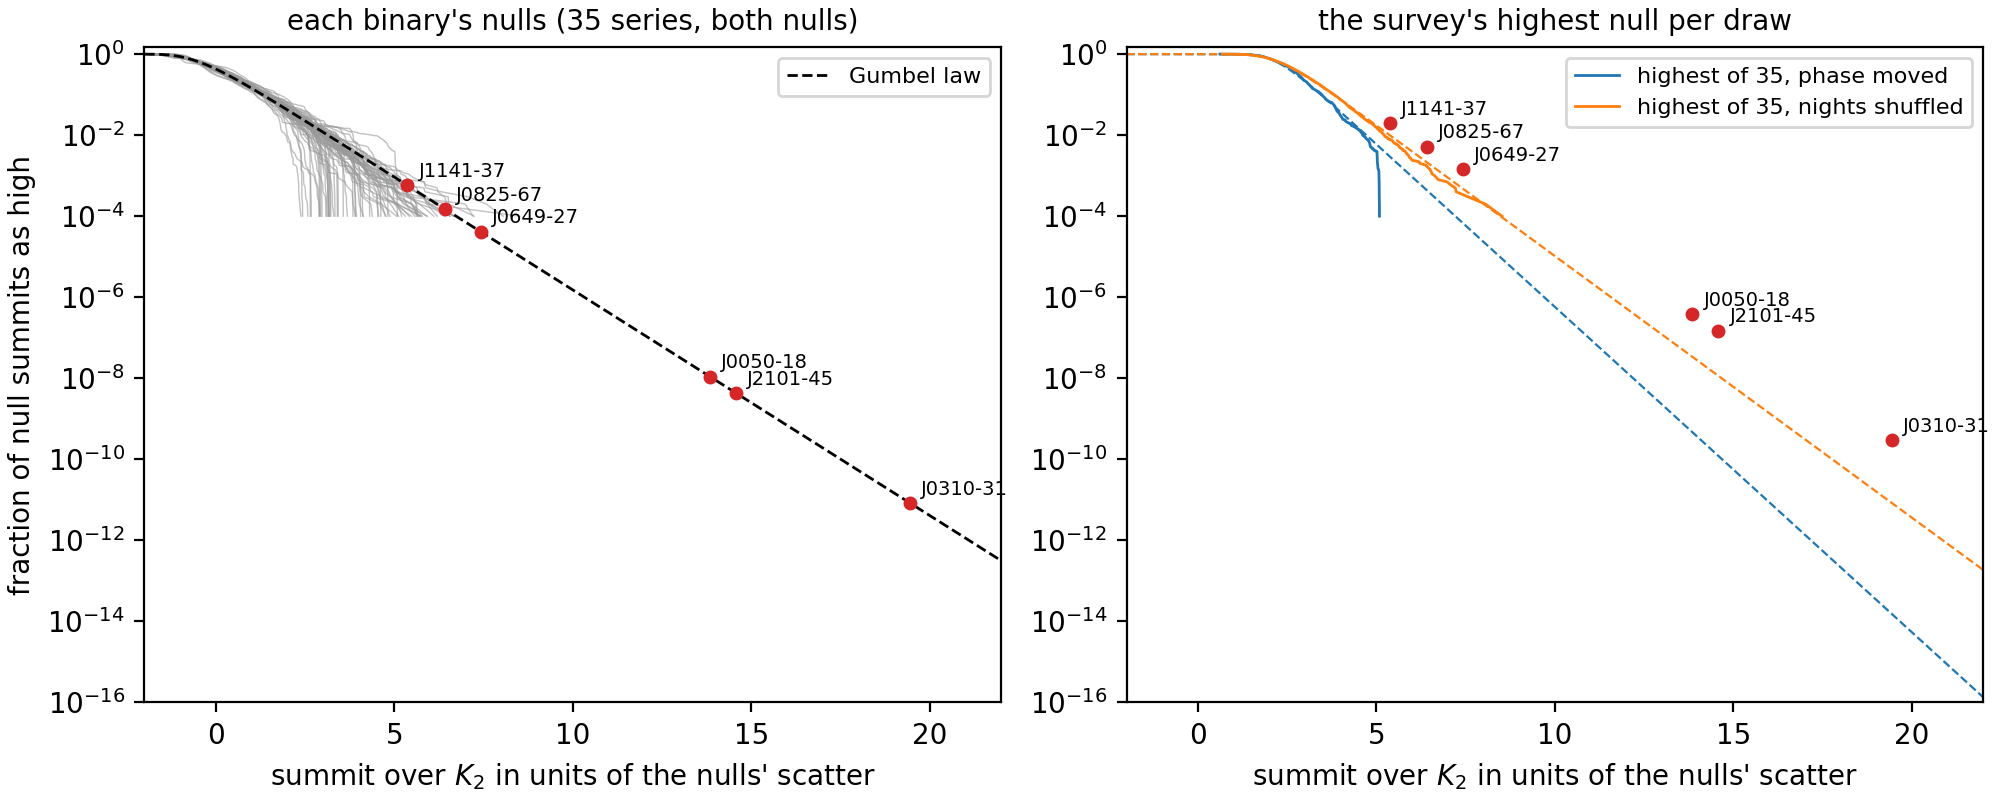
\includegraphics[width=\textwidth]{data/nulls.png}
\caption{Left: the fraction of each binary's $2\times10^4$ null summits at or above a given height
in units of their scatter, under both nulls, for the 35 binaries searched, against the Gumbel law
of unit scatter (dashed), with the six companions of the survey at their observed $z$ and
$p_\mathrm{G}$. Right: the same for the survey's highest null, the largest of the 35 standardised
null summits in each draw, with the Gumbel laws fitted to it (dashed) and the six companions at
their probabilities across the survey.}\label{fig:nulls}
\end{figure}

\subsection{EBLM J2101$-$45}

J2101$-$45's 75 spectra over 2298\,d give \Ktwo\ $= 65.41 \pm 0.32 \pm 0.32$\,\kms\ at an offset of
$+1.45$\,\kms\ (Table~\ref{tab:new}), the systematic term from its eight observing seasons. The
companion holds under every change of the analysis (Table~\ref{tab:robust}): the five variants
give 65.26 to 65.91\,\kms, within 1.1 times the total uncertainty of the measured value, the red
half of the band finds it at 21 and the blue half at 8 times the nulls' scatter, and the L\,98-59
template at 19. Three of its four parts by date find it on their own, at 6.5 to $9.8$ in the
nulls' units, at 65.41 to 66.16\,\kms; the fourth, at 1.1, does not. A companion injected at a flux
ratio of $10^{-3}$ is recovered at $65.61$\,\kms, and against it the real companion's lines match
the template's at $3.1\times10^{-3}$; one injected at $3\times10^{-4}$ is not recovered. The masses
are $m_1\sin^3 i = 1.415 \pm 0.024$ and $m_2\sin^3 i = 0.552 \pm 0.006$\,\Msun, and since the
binary eclipses, the primary's Gaia DR3 radius of $2.67$\,R$_\odot$ requires $\sin^3 i > 0.993$, so
the masses themselves are within 0.7 per cent of these. The primary, at $1.42$\,\Msun\ and
$2.67$\,R$_\odot$, lies above the main sequence. The model-based masses of
ref.~\cite{Triaud2017}, $1.29 \pm 0.10$ and $0.523 \pm 0.043$\,\Msun, differ from the dynamical
ones by 1.2 and 0.7 times the combined uncertainties.

\subsection{Three candidates}

J0649$-$27, J0825$-$67 and J1141$-$37 do not reach $5\sigma$ on their own nulls and fall to 2.1 to
$3.0\sigma$ across the survey, so their semi-amplitudes (Table~\ref{tab:new},
Fig.~\ref{fig:diagnostics}) are those their candidate companions would have. Each has a specific
weakness. One of the $10^4$ draws of J0649$-$27's adopted null reaches 6.7 times the nulls'
scatter, against its summit's 7.4; neither half of its 43 spectra finds the companion on its own, at 1.0 and
1.7 in the nulls' units; and the red half of the band, where an M dwarf's lines carry most of the
signal, peaks instead at $139.8$\,\kms\ and 2.8, while the blue half finds $120.35$\,\kms\ at 4.4.
J0825$-$67 rests on 27 spectra, too few for its parts or alternate nights to be measured alone, and
its uncertainty comes from its five seasons; companions injected along its moved track are not
recovered at either flux ratio, the summit falling at 94\,\kms\ and 0.7 to 0.9 in the nulls' units,
so its spectra do not test the method's recovery. J1141$-$37's 30 spectra divide into halves at 1.1
and 3.5 in the nulls' units and alternate nights at 5.5 and 0.9, and its seasons give a systematic
uncertainty of 2.6\,\kms. For J0649$-$27 and J1141$-$37 the injections at $10^{-3}$ are recovered
within 0.15\,\kms, and against them the candidate companions' lines would match the template's at
$0.7\times10^{-3}$, the order expected for an M3 dwarf beside an F star. The model-based masses of
ref.~\cite{Triaud2017} for J0649$-$27, $1.45 \pm 0.13$ and $0.371 \pm 0.061$\,\Msun, and for
J1141$-$37, $1.22 \pm 0.10$ and $0.354 \pm 0.050$\,\Msun, are consistent with the minimum masses
the candidates would give, $1.230 \pm 0.071$ and $0.335 \pm 0.012$, and $1.320 \pm 0.090$ and
$0.371 \pm 0.015$\,\Msun, which the eclipses bound by $\sin^3 i > 0.96$. More spectra of these
three would decide them.

\begin{table}[!htbp]
\centering
\caption{The 35 searchable EBLM binaries with archived HARPS series: the spectra (nights), the
span, the primary's orbit fitted to the measured velocities, and the summit of the trail over \Ktwo\
at a systemic offset of $+1.0$\,\kms\ with its $z$ and false-alarm probability. Companions at
$5\sigma$ or more are in bold and candidates between 3 and $5\sigma$ in italics.}\label{tab:survey}
\small
\begin{tabular}{lrrrrrrrr}
\toprule
EBLM & Spectra & Span (d) & $P$ (d) & \Kone\ (\kms) & $e$ & \Ktwo\ (\kms) & $z$ & $p_\mathrm{G}$\\
\midrule
\tabinput{data/tab_survey.tex}
\bottomrule
\end{tabular}
\end{table}

\begin{table}[!htbp]
\centering
\caption{J2101$-$45 and the three candidates, measured with the offset free: the semi-amplitude
with its statistical and systematic uncertainties, the offset with the 16th to 84th percentiles of
300 draws of whole nights, the false-alarm probability with its Gaussian significance on the
binary's own nulls and across the survey, and the minimum masses with the total uncertainty of
\Ktwo\ carried through.}\label{tab:new}
\footnotesize\setlength{\tabcolsep}{2pt}
\resizebox{\textwidth}{!}{%
\begin{tabular}{lcccccc}
\toprule
EBLM & \Ktwo\ (\kms) & \dvsys\ (\kms) & $p_\mathrm{G}$ ($\sigma$) & Across 35 ($\sigma$) & $m_1\sin^3 i$ (\Msun) & $m_2\sin^3 i$ (\Msun)\\
\midrule
\tabinput{data/tab_new.tex}
\bottomrule
\end{tabular}}
\end{table}

\begin{table}[!htbp]
\centering
\caption{The semi-amplitude, with the summit's $z$ in brackets, as measured and under the five
changes of the analysis of Section~\ref{sec:robust}: three and eight principal components, the
template kept blueward or redward of 5500\,\AA, and the template from L\,98-59's spectra.}\label{tab:robust}
\footnotesize\setlength{\tabcolsep}{3pt}
\begin{tabular}{lcccccc}
\toprule
System & As measured & 3 components & 8 components & 3800--5500\,\AA & 5500--7880\,\AA & L\,98-59\\
\midrule
\tabinput{data/tab_robust.tex}
\bottomrule
\end{tabular}
\end{table}

\begin{table}[!htbp]
\centering
\caption{Companions injected into the spectra a quarter of a period from the real ones: the
flux ratio and \Ktwo\ injected, the semi-amplitude and offset recovered along the moved track with
the summit's $z$, and, where the injection at $10^{-3}$ is recovered, the flux ratio at which the
real companion's lines match the template's ($10^{-3}$).}\label{tab:inject}
\small
\begin{tabular}{lcccccc}
\toprule
System & Flux ratio & \Ktwo\ injected & \Ktwo\ recovered & \dvsys\ (\kms) & $z$ & Real companion\\
\midrule
\tabinput{data/tab_inject.tex}
\bottomrule
\end{tabular}
\end{table}

\begin{figure}[!htbp]
\centering
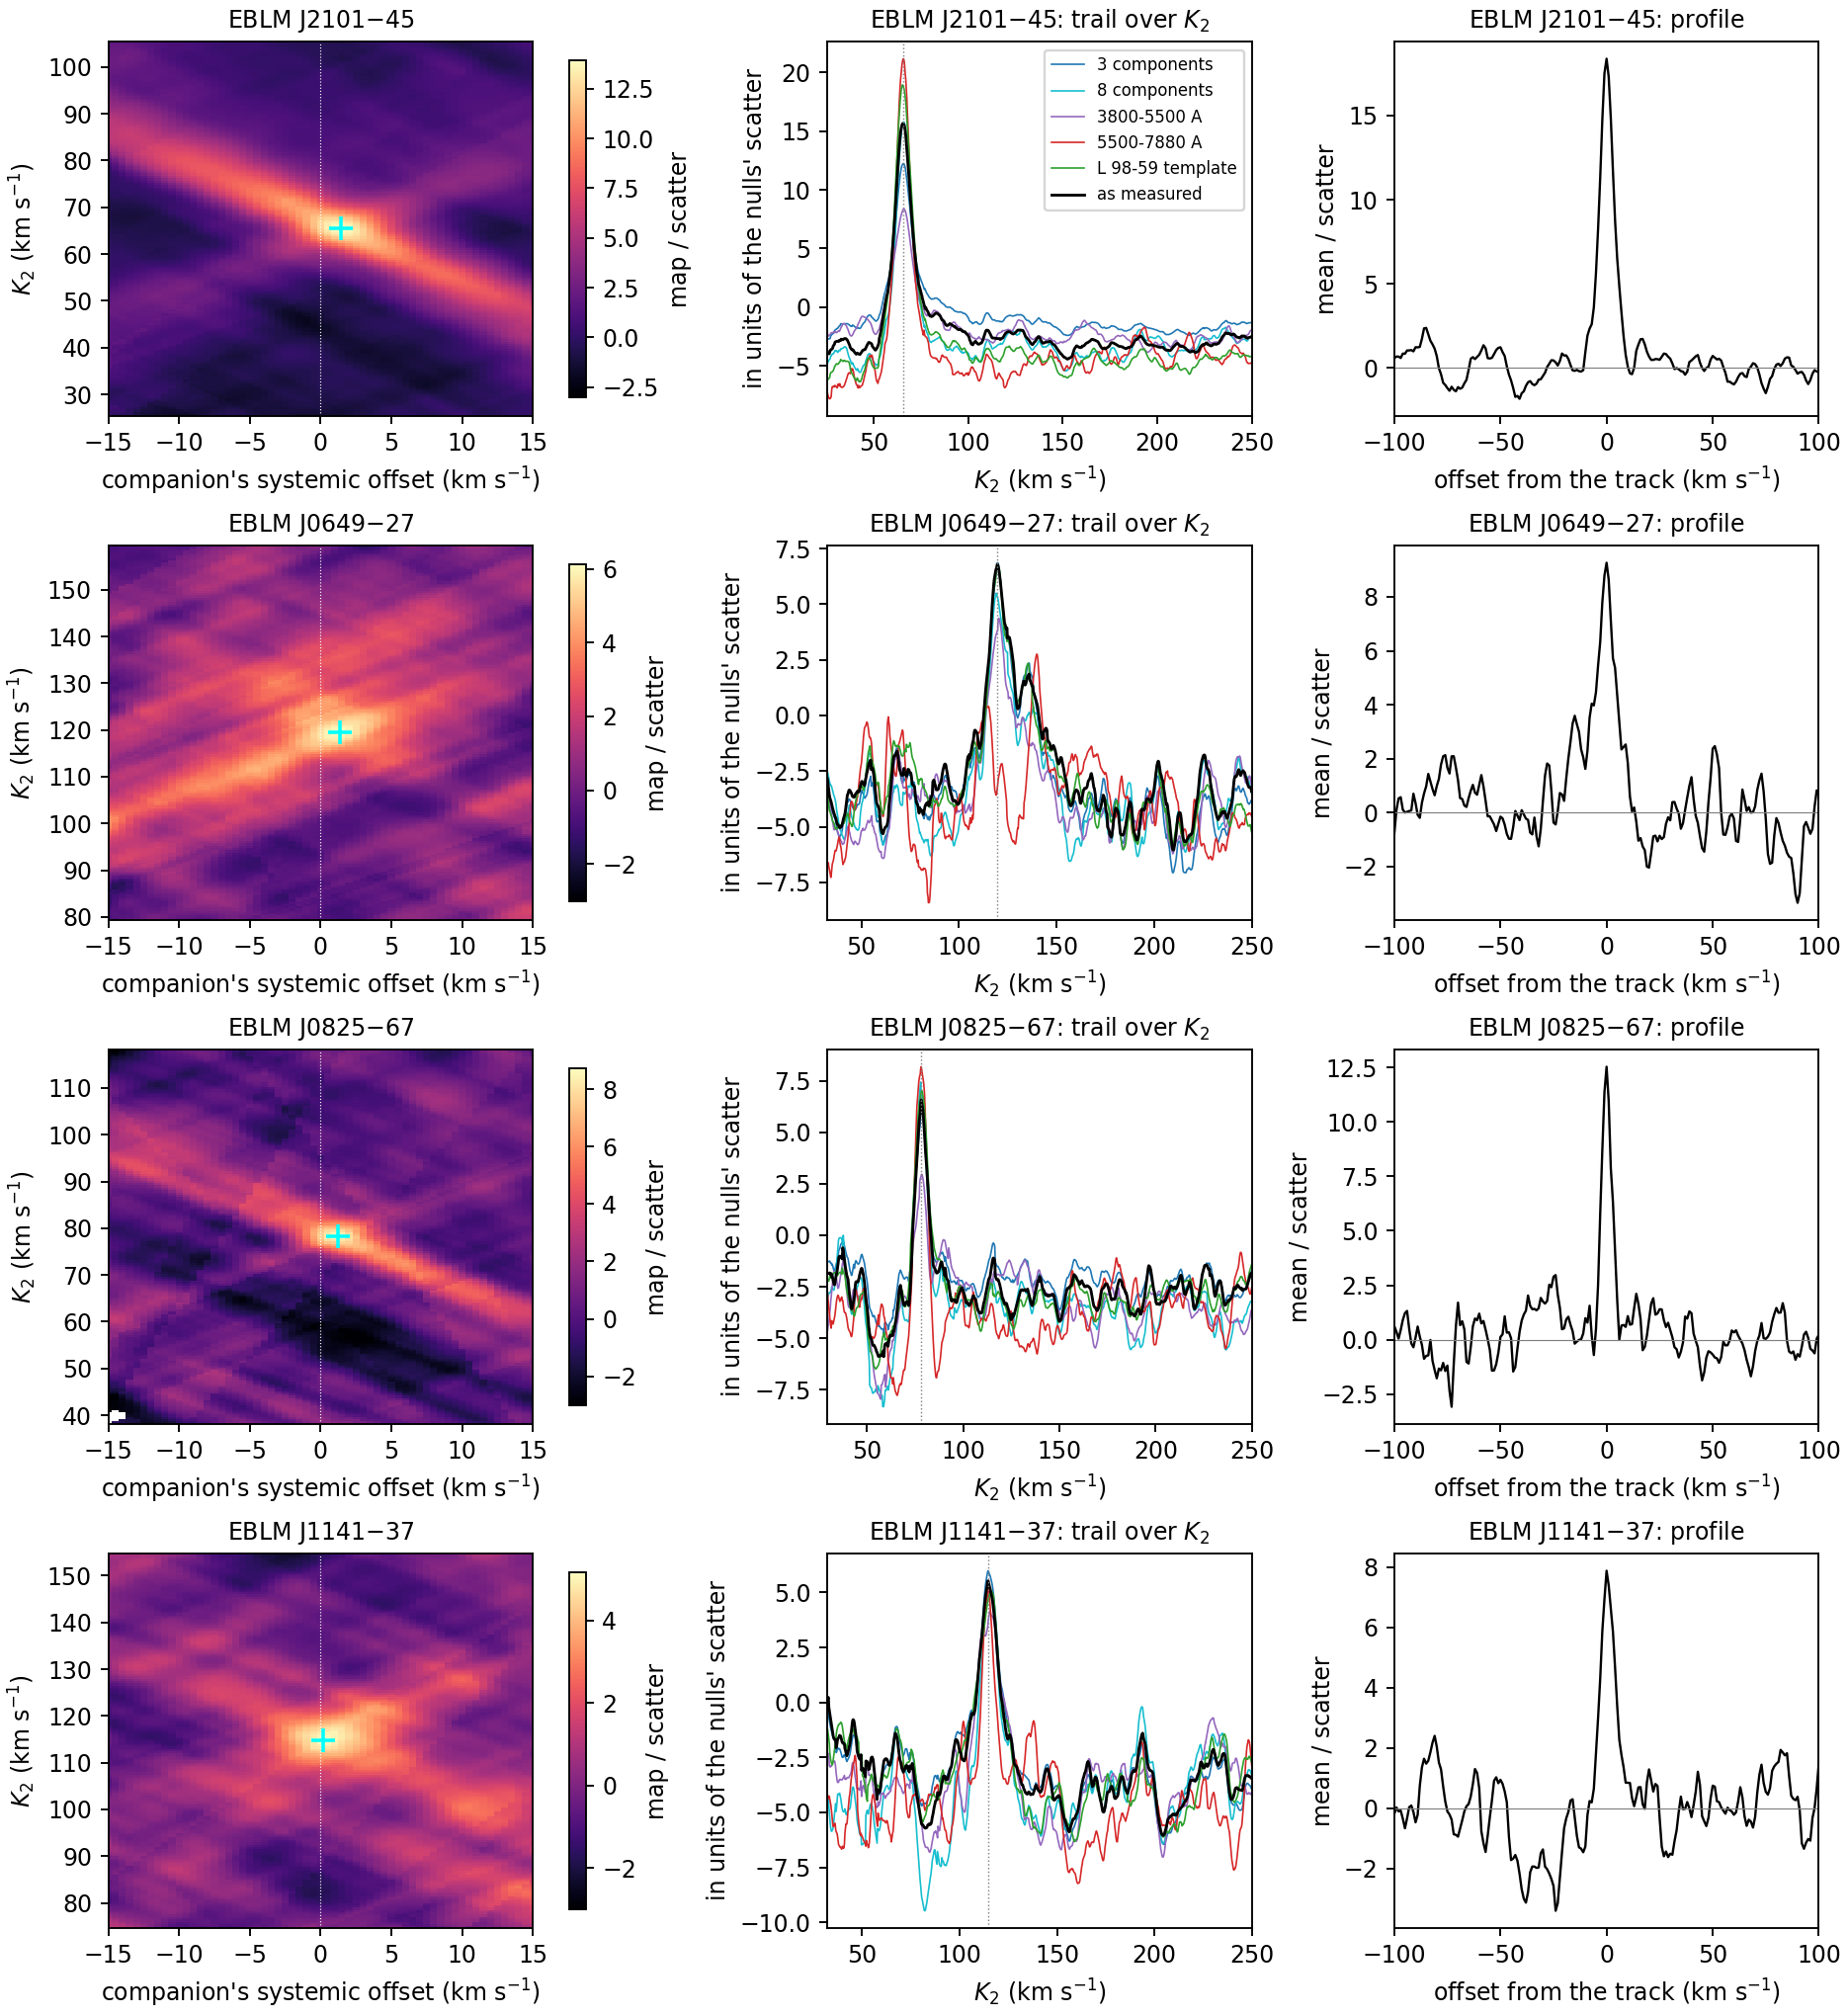
\includegraphics[width=\textwidth]{data/diagnostics.png}
\caption{J2101$-$45 and the three candidates. Left: the map over \Ktwo\ and the companion's
systemic offset in units of its scatter, the cross at the peak. Middle: the trail over \Ktwo\ at
the peak's offset in units of the stricter null's scatter, as measured (black) and under the five
changes of the analysis. Right: the cleaned rows summed in the companion's frame at the peak, in
units of the profile's scatter beyond 30\,\kms.}\label{fig:diagnostics}
\end{figure}

\section{Beyond the catalogue orbits}\label{sec:wider}

\subsection{Eight more HARPS binaries}

The selection of Section~\ref{sec:data} needs an orbit from Gaia DR3 or SB9. The ESO archive holds
HARPS series of 41 further EBLM binaries with 15 or more spectra above a signal-to-noise ratio of
10, and for these the orbit is fitted to the series' own velocities: each spectrum's velocity is
measured against GJ\,367's line depths, a circular-orbit periodogram and a Keplerian fit give the
orbit, the primary's own line depths are made from its spectra at that orbit's velocities and the
velocities measured again against them, twice, and the fit that leaves the least scatter is kept.
The 41 series were searched along their orbits, and the eight in which a companion appears were
built, measured and calibrated as in Section~\ref{sec:method}, the offset held at $+1.0$\,\kms\
for the calibration. Since the 41 were searched together, each binary's own $p_\mathrm{G}$ is
compounded over them, $1-(1-p_\mathrm{G})^{41}$ (Table~\ref{tab:wider}).

Four companions stand at $5\sigma$ or more across the 41: J2122$-$32, J0425$-$46, J2054$-$32 and
J0535$-$08, at 5.3 to $5.7\sigma$, with \Ktwo\ measured to 0.2 to 0.6 per cent and offsets of
$+0.90$ to $+1.15$\,\kms, as in the systems of Section~\ref{sec:validation}. None has a published
double-lined solution, and Gaia DR3 holds single-lined orbits alone for J2054$-$32 and
J0425$-$46~\cite{GaiaNSS2023}. J0345$-$10, the binary TOI-395, reaches $4.1\sigma$ on its own nulls
and $3.2\sigma$ across the 41, and J1204$-$47, J1328$+$05 and J0610$-$56 reach 3.0 to $3.3\sigma$
alone; these four remain candidates, J1204$-$47 with a semi-amplitude its NIRPS spectra repeat
(Section~\ref{sec:nir}).

\begin{table}[!htbp]
\centering
\caption{The eight companions among the 41 EBLM binaries whose orbits are fitted to their own HARPS
velocities: the spectra (nights), the orbit, the semi-amplitude with its statistical and
systematic uncertainties, the offset with the 16th to 84th percentiles of 300 draws of whole
nights, the false-alarm probability with its Gaussian significance on the binary's own nulls at an
offset of $+1.0$\,\kms\ and compounded over the 41, and the minimum masses. Companions at $5\sigma$
or more across the 41 are in bold. J1328$+$05's 21 spectra are too few for a systematic
term.}\label{tab:wider}
\footnotesize\setlength{\tabcolsep}{2pt}
\resizebox{\textwidth}{!}{%
\begin{tabular}{lcccccccccc}
\toprule
EBLM & Spectra & $P$ (d) & \Kone\ (\kms) & $e$ & \Ktwo\ (\kms) & \dvsys\ (\kms) & $p_\mathrm{G}$ ($\sigma$) & Across 41 ($\sigma$) & $m_1\sin^3 i$ (\Msun) & $m_2\sin^3 i$ (\Msun)\\
\midrule
\tabinput{data/tab_wider.tex}
\bottomrule
\end{tabular}}
\end{table}

\subsection{The near infrared}\label{sec:nir}

NIRPS~\cite{Bouchy2017} has observed most of these binaries alongside HARPS since 2023, and in the
near infrared an M dwarf carries a larger share of the light. Twenty of the EBLM binaries with a
HARPS orbit have NIRPS series long enough to search, from the archive's telluric-corrected
products. Three steps change in this band. A solar-type primary has too few lines in it for each
spectrum to be placed on its own, so each is put at the velocity of the HARPS orbit and left
unaligned. Before each residual's cubic is removed, the telluric bands and the samples where the
series' median spectrum falls to 0.2 or below are set aside, since the ratio to a median near zero
would otherwise dominate the fit. The template is the line depths of GJ\,581~\cite{Bonfils2005} from
its 40 best NIRPS spectra, depths above 0.8, which lie at the edges of the telluric bands, removed,
and the template moved by $-2.01$\,\kms\ onto the laboratory wavelengths of the Kurucz line
list~\cite{Kurucz2011}. With this template the three best-measured companions, J1540$-$09's,
J1613$-$76's and J1204$-$47's, sit at offsets of $+3.70$, $+4.45$ and $+0.85$\,\kms, too far apart
to hold one offset, so the probabilities are quoted with the offset free within 10\,\kms\ of zero
and compounded over the 20 series (Table~\ref{tab:nirps}).

J1540$-$09's companion, measured by EBLM~XX at \Ktwo\ $= 60.03 \pm 0.26$\,\kms~\cite{Stevenson2026},
is recovered from 118 NIRPS spectra at $59.98 \pm 0.50 \pm 0.78$\,\kms\ and $4.0\sigma$. J1928$-$38's
39 NIRPS spectra put its companion at $62.07 \pm 2.79 \pm 1.53$\,\kms\ against EBLM~XX's $64.35 \pm
2.82$, at $1.4\sigma$, where its 74 HARPS spectra show nothing (Section~\ref{sec:validation}).
J1613$-$76, whose HARPS series shows no companion, gives one at $70.11 \pm 1.76 \pm 3.02$\,\kms\ and
$3.5\sigma$ from 22 spectra, a candidate, and J1204$-$47's NIRPS spectra repeat its HARPS
semi-amplitude within 0.6\,\kms. J0353$-$16 and J0055$-$00 reach 2.0 and $1.2\sigma$.

\begin{table}[!htbp]
\centering
\caption{The NIRPS series in which a companion appears: the spectra (nights), the semi-amplitude
with its statistical and systematic uncertainties, the offset with the 16th to 84th percentiles of
300 draws of whole nights, the false-alarm probability with the offset free within 10\,\kms\ on the
binary's own nulls and compounded over the 20 series searched, the companion's minimum mass, and
the semi-amplitude measured elsewhere.}\label{tab:nirps}
\footnotesize\setlength{\tabcolsep}{2pt}
\resizebox{\textwidth}{!}{%
\begin{tabular}{lccccccc}
\toprule
EBLM & Spectra & \Ktwo\ (\kms) & \dvsys\ (\kms) & $p_\mathrm{G}$ ($\sigma$) & Across 20 ($\sigma$) & $m_2\sin^3 i$ (\Msun) & \Ktwo\ elsewhere (\kms)\\
\midrule
\tabinput{data/tab_nirps.tex}
\bottomrule
\end{tabular}}
\end{table}

\subsection{Masses and radii from the eclipses}\label{sec:eclipse}

The binaries eclipse, and TESS~\cite{Ricker2015} light curves, SPOC's at the shortest cadence or
else TESS-SPOC's or QLP's read through Lightkurve~\cite{Lightkurve2018}, give the inclination and
the radii. Both eclipses are modelled where the spectroscopic orbit places them, $e$ and $\omega$
held at the orbit's: the transit is a dark disk of radius ratio $R_2/R_1$ across a quadratically
limb-darkened primary, parametrised by $q_1$ and $q_2$~\cite{Kipping2013}, diluted by the
companion's share $L_2$ of the TESS-band light, and the occultation removes $L_2$ times the hidden
fraction of the companion's disk, its limb darkening held at 0.4 and 0.3; each exposure is
integrated over its length. The time of periastron, the period, $R_2/R_1$, $a/R_1$, $\cos i$,
$q_1$, $q_2$ and $L_2$ are fitted from several starts, small and grazing, by least squares and
sampled with emcee~\cite{ForemanMackey2013}, the primary's radius held to its TIC
value~\cite{Stassun2019} within 7 per cent except for J0535$-$08 and J0345$-$10. The inclination
turns the minimum masses into masses, and $a/R_1$ with $a\sin i = (K_1+K_2)P\sqrt{1-e^2}/2\pi$ gives
both radii (Table~\ref{tab:eclipse}).

J0535$-$08's eclipses, 18.3 and 2.7 per cent deep at an impact parameter of 0.19, give masses of
$0.970 \pm 0.011$ and $0.521 \pm 0.003$\,\Msun\ and radii of 1.209 and 0.505\,R$_\odot$, both
stars to within one per cent without the TIC radius. In J2122$-$32 the companion passes clear of
the primary at conjunction, its impact parameter 1.76 against $1 + R_2/R_1 = 1.48$, and only its
occultation, 1.3 per cent deep, is seen; J2054$-$32, J0345$-$10 and J1328$+$05 graze, so their
companions' radii stay loose while their masses, with $\sin^3 i$ between 0.976 and 0.997, do not.
J1613$-$76's points scatter 2.5 times their errors about the model, which understates its radius
intervals by that factor. J0425$-$46's primary has left the main sequence, at 1.59\,\Msun\ and
3.21\,R$_\odot$, beside a companion of 0.743\,\Msun\ and 0.704\,R$_\odot$.

\begin{table}[!htbp]
\centering
\caption{Masses and radii of the binaries of Tables~\ref{tab:wider} and~\ref{tab:nirps} from their
TESS eclipses: the transit and occultation windows observed, the inclination with its 16th to 84th
percentiles, the companion's share of the TESS-band light, the masses with the semi-amplitude's
total uncertainty carried through, and the radii with the eclipse fit's percentiles. J1613$-$76's
\Ktwo\ is its NIRPS value and the others' their HARPS values; the masses of the candidates are
those their companions would have.}\label{tab:eclipse}
\footnotesize\setlength{\tabcolsep}{3pt}
\resizebox{\textwidth}{!}{%
\begin{tabular}{lccccccc}
\toprule
EBLM & Windows & $i$ (deg) & $L_2$ & $M_1$ (\Msun) & $M_2$ (\Msun) & $R_1$ (R$_\odot$) & $R_2$ (R$_\odot$)\\
\midrule
\tabinput{data/tab_eclipse.tex}
\bottomrule
\end{tabular}}
\end{table}

\section{Discussion}\label{sec:discussion}

The semi-amplitudes measured here differ from the published ones by $-0.15$ to $+0.16$\,\kms,
within the published uncertainties, although the analysis makes its own choice at each step. The
template is an observed M1\,V spectrum rather than a line mask or a synthetic spectrum; the
primary's spectrum is removed by division by the series' median in the primary's frame and by
principal components of the cross-correlation rows, rather than by a singular value decomposition
of the spectra; the significance is measured against nulls built from the same rows rather than
from a fit to the map; and the uncertainty comes from resampling whole nights and dividing the
series by date. The agreement indicates that the published dynamical masses of TOI-1338 and EBLM
J0310$-$31 do not depend on those analysis choices at the level of their quoted uncertainties, and
that the near-infrared semi-amplitude of HD\,4875's companion holds in the optical.

The calibration separates the height of a summit from its probability. In units of the nulls'
scatter the four companions stand 13.8 to 19.4 high, but the nulls are drawn $10^4$ times each, so
the empirical probability stops at $10^{-4}$, and beyond it the probability rests on the Gumbel
law. That law fits the nulls to the depth they reach, and for the four companions the fitted
tails are as light as Gumbel's or lighter, so their probabilities are not optimistic. Their
summits also stand 11 to 16 times the nulls' scatter beyond the highest of the adopted null's
$10^4$ draws.
Across the survey the probability of the weakest of the four, HD\,4875, is $4\times10^{-7}$,
and for J2101$-$45 $1.5\times10^{-7}$. The three candidates show why the survey-wide accounting
matters: at 3.3 to $3.9\sigma$ alone they would each look like detections, and 35 binaries searched
over \Ktwo\ make summits of that height expected.

The archive's own completeness matters as much as the method. It holds 114 HARPS spectra of
J0310$-$31 above a signal-to-noise ratio of 10, against the 71 of the published analysis, and 260
usable ESPRESSO spectra of TOI-1338, two and a half times the published set. A detection's
significance grows with the square root of the number of spectra at fixed quality, and the
candidates, with 27 to 43 spectra, are where more spectra would count.

The method has the limits of any optical analysis of these binaries. Toward 0.1\,\Msun\ the
companion's optical flux falls to $10^{-4}$ of the primary's and below, and the HARPS series of
J1928$-$38 and of the lowest-mass companions do not reach them; no injection at
$3\times10^{-4}$ is detected, and only J1141$-$37's returns the injected \Ktwo, at 1.8 in the
nulls' units. The near infrared carries a larger share of the
companion's light, and there the method recovers J1540$-$09's published companion and reaches
J1928$-$38's and J1613$-$76's, which their HARPS series do not (Section~\ref{sec:nir}).

\section{Conclusion}\label{sec:conclusion}

An analysis of public ESO archive spectra, independent of the published pipelines, recovers the
M-dwarf companions of TOI-1338, EBLM J0310$-$31 and HD\,4875 with false-alarm probabilities of
$10^{-11}$, $8\times10^{-12}$ and $1\times10^{-8}$ and measures their semi-amplitudes as $77.27 \pm
0.18$, $88.12 \pm 0.38$ and $75.29 \pm 0.93$\,\kms, within $0.16$\,\kms\ of the published values,
with masses within 0.6 per cent of the published dynamical masses. HD\,4875's companion, measured
before in the near-infrared alone, is detected here in the optical. The companion's lines sit
$+1.05$ to $+1.25$\,\kms\ from the primary's systemic velocity in all three, and leaving that offset
free is needed for accuracy at the tenth of a kilometre per second. Across the 35 searchable
southern EBLM binaries with archived HARPS series, the companion of EBLM J2101$-$45 is measured for
the first time, at a false-alarm probability of $1.5\times10^{-7}$ across the survey, with \Ktwo\
$= 65.41 \pm 0.46$\,\kms\ and minimum masses of $1.415$ and $0.552$\,\Msun; the companions of
J0649$-$27, J0825$-$67 and J1141$-$37 remain candidates. Among 41 EBLM binaries outside the
catalogue orbits, the companions of J2122$-$32, J0425$-$46, J2054$-$32 and J0535$-$08 are measured
for the first time at 5.3 to $5.7\sigma$ across the 41, and with their TESS eclipses their masses
and radii follow without stellar models; NIRPS spectra recover J1540$-$09's companion within
0.05\,\kms\ of its published semi-amplitude.

\section*{Acknowledgements}

Based on data obtained from the ESO Science Archive Facility, from ESO programmes
092.D-0261(A), 095.C-0367(A), 099.C-0138(A), 099.C-0138(B), 0101.C-0510(C), 103.2024.001,
106.212H.001, 106.212H.007, 106.212H.009, 106.212H.010, 106.216B.001, 106.216B.002, 106.216B.003,
106.21TJ.001, 1101.C-0721(A), 112.25GZ.001, 112.25GZ.002, 112.25GZ.003, 112.25GZ.004,
112.25KP.001, 112.25UD.001, 113.26NT.001, 115.27V0.001, 115.27V0.002, 116.28LH.001, 116.28LL.001
and 116.28LL.002.
This work has made use of data from the European Space Agency mission Gaia, processed by the Gaia
Data Processing and Analysis Consortium, funded by national institutions, in particular the
institutions participating in the Gaia Multilateral Agreement; of the SIMBAD database and the
VizieR catalogue access tool, operated at CDS, Strasbourg, France; and of the SB9 catalogue of
spectroscopic binary orbits.

\section*{Data availability}

The spectra are public in the ESO Science Archive. The analysis is the binaries approach of the
seti-tools package that holds this paper (\texttt{seti.py composition binaries}, whose modes build
the rows, search, calibrate and measure), and its coverage store records the run as
\texttt{binaries\_eblm\_known\_orbits}. The paper's data folder holds the measurements and their
maps, curves and profiles, the robustness and injection measurements, the calibrations, the
survey's search results, the eclipse fits, and the tables written from them.

\begin{thebibliography}{99}\small\raggedright
\setlength{\itemsep}{1pt}

\bibitem{Torres2010}
G.~Torres, J.~Andersen and A.~Gim\'enez, Accurate masses and radii of normal stars: modern
results and applications, \emph{Astron. Astrophys. Rev.} \textbf{18}, 67 (2010).

\bibitem{Southworth2015}
J.~Southworth, DEBCat: a catalogue of detached eclipsing binary stars, in \emph{Living Together:
Planets, Host Stars and Binaries}, ASP Conf. Ser. \textbf{496}, 164 (2015).

\bibitem{Triaud2013}
A.~H.~M.~J. Triaud et al., The EBLM project I. Physical and orbital parameters, including
spin-orbit angles, of two low-mass eclipsing binaries on opposite sides of the brown dwarf limit,
\emph{Astron. Astrophys.} \textbf{549}, A18 (2013).

\bibitem{Triaud2017}
A.~H.~M.~J. Triaud et al., The EBLM Project IV. Spectroscopic orbits of over 100 eclipsing M
dwarfs masquerading as transiting hot-Jupiters, \emph{Astron. Astrophys.} \textbf{608}, A129
(2017).

\bibitem{Maxted2023}
P.~F.~L. Maxted, A.~H.~M.~J. Triaud and D.~V. Martin, The EBLM Project: from false positives to
benchmark stars and circumbinary exoplanets, \emph{Universe} \textbf{9}, 498 (2023).

\bibitem{Martin2019}
D.~V. Martin et al., The BEBOP radial-velocity survey for circumbinary planets I. Eight years of
CORALIE observations of 47 single-line eclipsing binaries and abundance constraints on the masses
of circumbinary planets, \emph{Astron. Astrophys.} \textbf{624}, A68 (2019).

\bibitem{Standing2022}
M.~R. Standing et al., BEBOP II: sensitivity to sub-Saturn circumbinary planets using
radial-velocities, \emph{Mon. Not. R. Astron. Soc.} \textbf{511}, 3571 (2022).

\bibitem{Triaud2022}
A.~H.~M.~J. Triaud et al., BEBOP III. Observations and an independent mass measurement of
Kepler-16 (AB) b, the first circumbinary planet detected with radial velocities, \emph{Mon. Not.
R. Astron. Soc.} \textbf{511}, 3561 (2022).

\bibitem{Snellen2010}
I.~A.~G. Snellen, R.~J. de Kok, E.~J.~W. de Mooij and S.~Albrecht, The orbital motion, absolute
mass and high-altitude winds of exoplanet HD\,209458b, \emph{Nature} \textbf{465}, 1049 (2010).

\bibitem{Brogi2012}
M.~Brogi et al., The signature of orbital motion from the dayside of the planet $\tau$ Bo\"otis b,
\emph{Nature} \textbf{486}, 502 (2012).

\bibitem{Kostov2020}
V.~B. Kostov et al., TOI-1338: TESS' first transiting circumbinary planet, \emph{Astron. J.}
\textbf{159}, 253 (2020).

\bibitem{Standing2023}
M.~R. Standing et al., Radial-velocity discovery of a second planet in the TOI-1338/BEBOP-1
circumbinary system, \emph{Nat. Astron.} \textbf{7}, 702 (2023).

\bibitem{Sebastian2024b}
D.~Sebastian et al., The EBLM project XIII. The absolute dynamical masses of the circumbinary
planet host TOI-1338/BEBOP-1, \emph{Mon. Not. R. Astron. Soc.} \textbf{530}, 2572 (2024).

\bibitem{Sebastian2024a}
D.~Sebastian, A.~H.~M.~J. Triaud and M.~Brogi, Saltire: a model to measure dynamical masses for
high-contrast binaries and exoplanets with high-resolution spectroscopy, \emph{Mon. Not. R.
Astron. Soc.} \textbf{527}, 10921 (2024).

\bibitem{Sebastian2025b}
D.~Sebastian et al., EBLM XV. Revised dynamical masses for the circumbinary planet host Kepler-16
AB, using the SOPHIE spectrograph, \emph{Mon. Not. R. Astron. Soc.} \textbf{540}, 2914 (2025).

\bibitem{Baycroft2025}
T.~A. Baycroft et al., BEBOP VII. SOPHIE discovery of BEBOP-3b, a circumbinary giant planet on an
eccentric orbit, \emph{Mon. Not. R. Astron. Soc.} \textbf{541}, 2801 (2025).

\bibitem{Stevenson2026}
A.~T. Stevenson et al., The EBLM project XX. Absolute dynamical masses of five low-mass eclipsing
binaries, and an evaluation of mass estimation methods, \emph{Mon. Not. R. Astron. Soc.}, in press
(2026), doi:10.1093/mnras/stag1904, arXiv:2610.18339.

\bibitem{Maxted2022}
P.~F.~L. Maxted et al., Fundamental effective temperature measurements for eclipsing binary
stars III. SPIRou near-infrared spectroscopy and CHEOPS photometry of the benchmark G0V star EBLM
J0113+31, \emph{Mon. Not. R. Astron. Soc.} \textbf{513}, 6042 (2022).

\bibitem{Sebastian2025a}
D.~Sebastian, A.~H.~M.~J. Triaud, P.~F.~L. Maxted and M.~Brogi, Accurate dynamical masses from
binaries with extreme brightness ratios, \emph{Contrib. Astron. Obs. Skalnat\'e Pleso}
\textbf{55}, 412 (2025).

\bibitem{Adshead2026}
N.~J. Adshead, P.~F.~L. Maxted and A.~Hahlin, Fundamental effective temperature measurements for
eclipsing binary stars VIII. NIRPS spectroscopy of CD$-$27\,2812, \emph{Mon. Not. R. Astron.
Soc.}, in press (2026), arXiv:2604.13631.

\bibitem{Hahlin2026}
A.~Hahlin et al., Fundamental effective temperature measurements for eclipsing binary stars IX.
Characterisation of 5 solar-type eclipsing binaries with M-dwarf companions, \emph{Mon. Not. R.
Astron. Soc.}, in press (2026), arXiv:2609.01033.

\bibitem{orbitlight}
orbitlight: planets, their atmospheres and the companions of their stars read out of archived
high-resolution spectra, https://huggingface.co/datasets/phanerozoic/orbitlight (2026).

\bibitem{GaiaNSS2023}
Gaia Collaboration, F.~Arenou et al., Gaia Data Release 3. Stellar multiplicity, a teaser for the
hidden treasure, \emph{Astron. Astrophys.} \textbf{674}, A34 (2023).

\bibitem{Pourbaix2004}
D.~Pourbaix et al., SB9: the ninth catalogue of spectroscopic binary orbits, \emph{Astron.
Astrophys.} \textbf{424}, 727 (2004).

\bibitem{Lam2021}
K.~W.~F. Lam et al., GJ 367b: a dense, ultrashort-period sub-Earth planet transiting a nearby
red dwarf star, \emph{Science} \textbf{374}, 1271 (2021).

\bibitem{Cloutier2019}
R.~Cloutier et al., Characterization of the L 98-59 multi-planetary system with HARPS,
\emph{Astron. Astrophys.} \textbf{629}, A111 (2019).

\bibitem{Gumbel1958}
E.~J. Gumbel, \emph{Statistics of Extremes} (Columbia University Press, New York, 1958).

\bibitem{Coles2001}
S.~Coles, \emph{An Introduction to Statistical Modeling of Extreme Values} (Springer, London,
2001).

\bibitem{Sidak1967}
Z.~\v{S}id\'ak, Rectangular confidence regions for the means of multivariate normal
distributions, \emph{J. Am. Stat. Assoc.} \textbf{62}, 626 (1967).

\bibitem{Mayor2003}
M.~Mayor et al., Setting new standards with HARPS, \emph{The Messenger} \textbf{114}, 20 (2003).

\bibitem{Pepe2021}
F.~Pepe et al., ESPRESSO at VLT: on-sky performance and first results, \emph{Astron. Astrophys.}
\textbf{645}, A96 (2021).

\bibitem{Bouchy2017}
F.~Bouchy et al., Near-InfraRed Planet Searcher to join HARPS on the ESO 3.6-metre telescope,
\emph{The Messenger} \textbf{169}, 21 (2017).

\bibitem{Bonfils2005}
X.~Bonfils et al., The HARPS search for southern extra-solar planets VI. A Neptune-mass planet
around the nearby M dwarf Gl\,581, \emph{Astron. Astrophys.} \textbf{443}, L15 (2005).

\bibitem{Kurucz2011}
R.~L. Kurucz, Including all the lines, \emph{Can. J. Phys.} \textbf{89}, 417 (2011).

\bibitem{Ricker2015}
G.~R. Ricker et al., Transiting Exoplanet Survey Satellite, \emph{J. Astron. Telesc. Instrum.
Syst.} \textbf{1}, 014003 (2015).

\bibitem{Lightkurve2018}
Lightkurve Collaboration, Lightkurve: Kepler and TESS time series analysis in Python,
Astrophysics Source Code Library, ascl:1812.013 (2018).

\bibitem{Kipping2013}
D.~M. Kipping, Efficient, uninformative sampling of limb darkening coefficients for two-parameter
laws, \emph{Mon. Not. R. Astron. Soc.} \textbf{435}, 2152 (2013).

\bibitem{ForemanMackey2013}
D.~Foreman-Mackey, D.~W. Hogg, D.~Lang and J.~Goodman, emcee: the MCMC hammer, \emph{Publ. Astron.
Soc. Pac.} \textbf{125}, 306 (2013).

\bibitem{Stassun2019}
K.~G. Stassun et al., The revised TESS Input Catalog and Candidate Target List, \emph{Astron. J.}
\textbf{158}, 138 (2019).

\end{thebibliography}

\end{document}
